\documentclass[twoside]{article}

\usepackage{amsmath,amsthm,amssymb,graphicx}
\usepackage{hyperref}
\usepackage[numbers]{natbib}
\usepackage{float}
\usepackage{bbm}

\theoremstyle{definition}
\newtheorem{thm}{Theorem}[section]
\newtheorem{lem}[thm]{Lemma}
\newtheorem{prop}[thm]{Proposition}
\newtheorem{cor}[thm]{Corollary}
\newenvironment{pf}{{\noindent\sc Proof. }}{\qed}
\newenvironment{map}{\[\begin{array}{cccc}} {\end{array}\]}

\newcommand{\comment}[1]{}
\theoremstyle{definition}
\newtheorem*{defn}{Definition}
\newtheorem*{exmp}{Example}
\newtheorem*{prob}{Problem}

\theoremstyle{remark}
\newtheorem*{rem}{Remark}
\newtheorem*{note}{Note}
\newtheorem*{exer}{Exercise}

\setlength{\oddsidemargin}{0.25 in}
\setlength{\evensidemargin}{-0.25 in}
\setlength{\topmargin}{-0.6 in}
\setlength{\textwidth}{6.5 in}
\setlength{\textheight}{8.5 in}
\setlength{\headsep}{0.75 in}
\setlength{\parindent}{0 in}
\setlength{\parskip}{0.1 in}

\newcommand{\widgraph}[2]{\includegraphics[keepaspectratio,width=#1]{#2}}
\newcommand{\widgraphr}[3]{\includegraphics[keepaspectratio,width=#1,angle=#3]{#2}}

\newcommand{\lecture}[4]{
   \pagestyle{myheadings}
   \thispagestyle{plain}
   \newpage
   \setcounter{page}{1}
   \noindent
   \begin{center}
   \framebox{
      \vbox{\vspace{2mm}
    \hbox to 6.28in { {\bf Stat365/665 (Spring 2015) Data Mining and Machine Learning \hfill Lecture: #4} }
       \vspace{6mm}
       \hbox to 6.28in { {\Large \hfill #1  \hfill} }
       \vspace{6mm}
       \hbox to 6.28in { {\it Lecturer: #2 \hfill Scribe: #3} }
      \vspace{2mm}}
   }
   \end{center}
   \markboth{#1}{#1}
   \vspace*{4mm}
}


%%%%%%%
% Some commonly used notation
%%%%%%%

\def\R{{\mathbb R}}
\def\X{{\mathcal X}}
\def\Y{{\mathcal Y}}
\def\H{{\mathcal H}}
\def\E{{\mathbb E}}
\def\sign{{\rm sign}}

\newcommand{\percent}{$\%$}

\begin{document}

\lecture{Data Mining and Machine Learning}{Sahand Negahban}{Leon Lixing Yu}{16}
\section{Announcement}
Homework assigned.\\
Start thinking about projects.\\
\section{Today}
- Wrap-up soft-margin SVM.\\
- Statistical Learning theory.\\

\section{soft-margin SVM}
We know that
\[\hat W \in \underset{W}{\operatorname{argmin}} \frac{C}{n} \sum \phi(w^T x_i y_i) + \|w\|^2 \]
Last time we proved that through the K.K.T. conditions, we have:
\[ w = \sum_{i=1}^n \alpha_i x_i y_i \;\;\;\; \frac{C}{n} \geq \alpha_i \geq 0\]
We can re-write it in kernel form:
\[ w = \sum_{i=1}^n \alpha_i k(x_i,\bullet)y_i\]
The notion, $\phi(S)$ stands for the positive part of $(1-S)$, $S$ can be anything here.  we rephrase it in math notation:
\[\phi(S) = (1-S)_+\]
If $1-S$ is negative, then $\phi(S) = 0$.

\subsection{Margin Error}
Everything, that is a support vector, is a margin error.See below.\\
\begin{figure}[H]
\centering
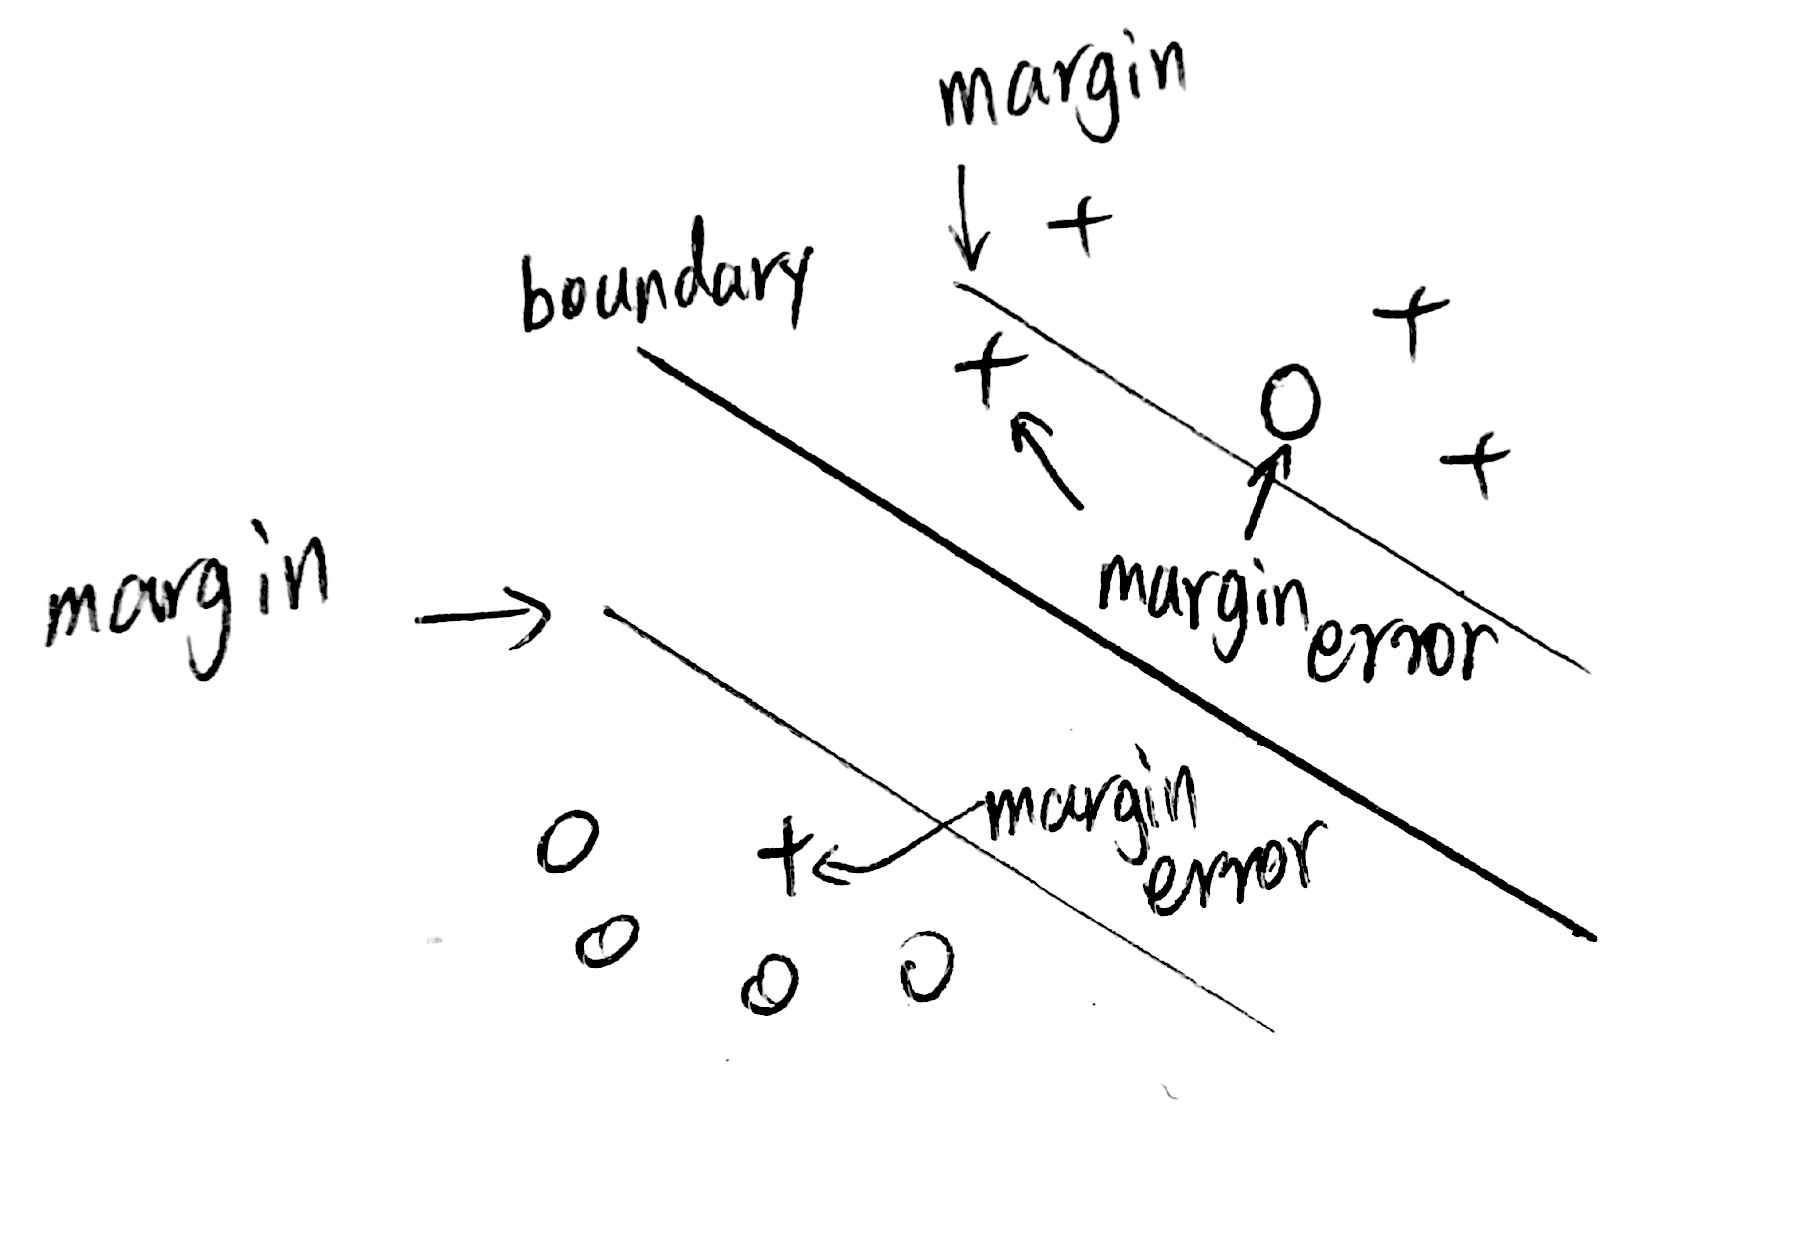
\includegraphics[width=120mm]{margin.jpg}
\caption{ Margin Error }
\end{figure}
Given $\|w\|^2$ controls the size of $w$, $\phi(w^T x_i y_i)$ controls the errors.\\
Also, remember that ideally we ant to control:
\[ \underset{w}{\operatorname{min}} \frac{C}{n} \sum_{i=1}^n \mathbbm{1} (w^T x_i y_i \leq 0) \;\;\;\;\; s.t. \; \|w\| \leq 1\]
The form above simply means that $\frac{1}{n}$ multiplied by the total number of errors is the average number of errors. However, it takes long time to compute (a.k.a: computatinally intractable). \\
For that reason, we use convex relaxation. 
\subsection{Convex Relaxation}
Say we have:
\[ w^T x_i, y_i =S\]
and its graph is given by:\\
\begin{figure}[H]
\centering
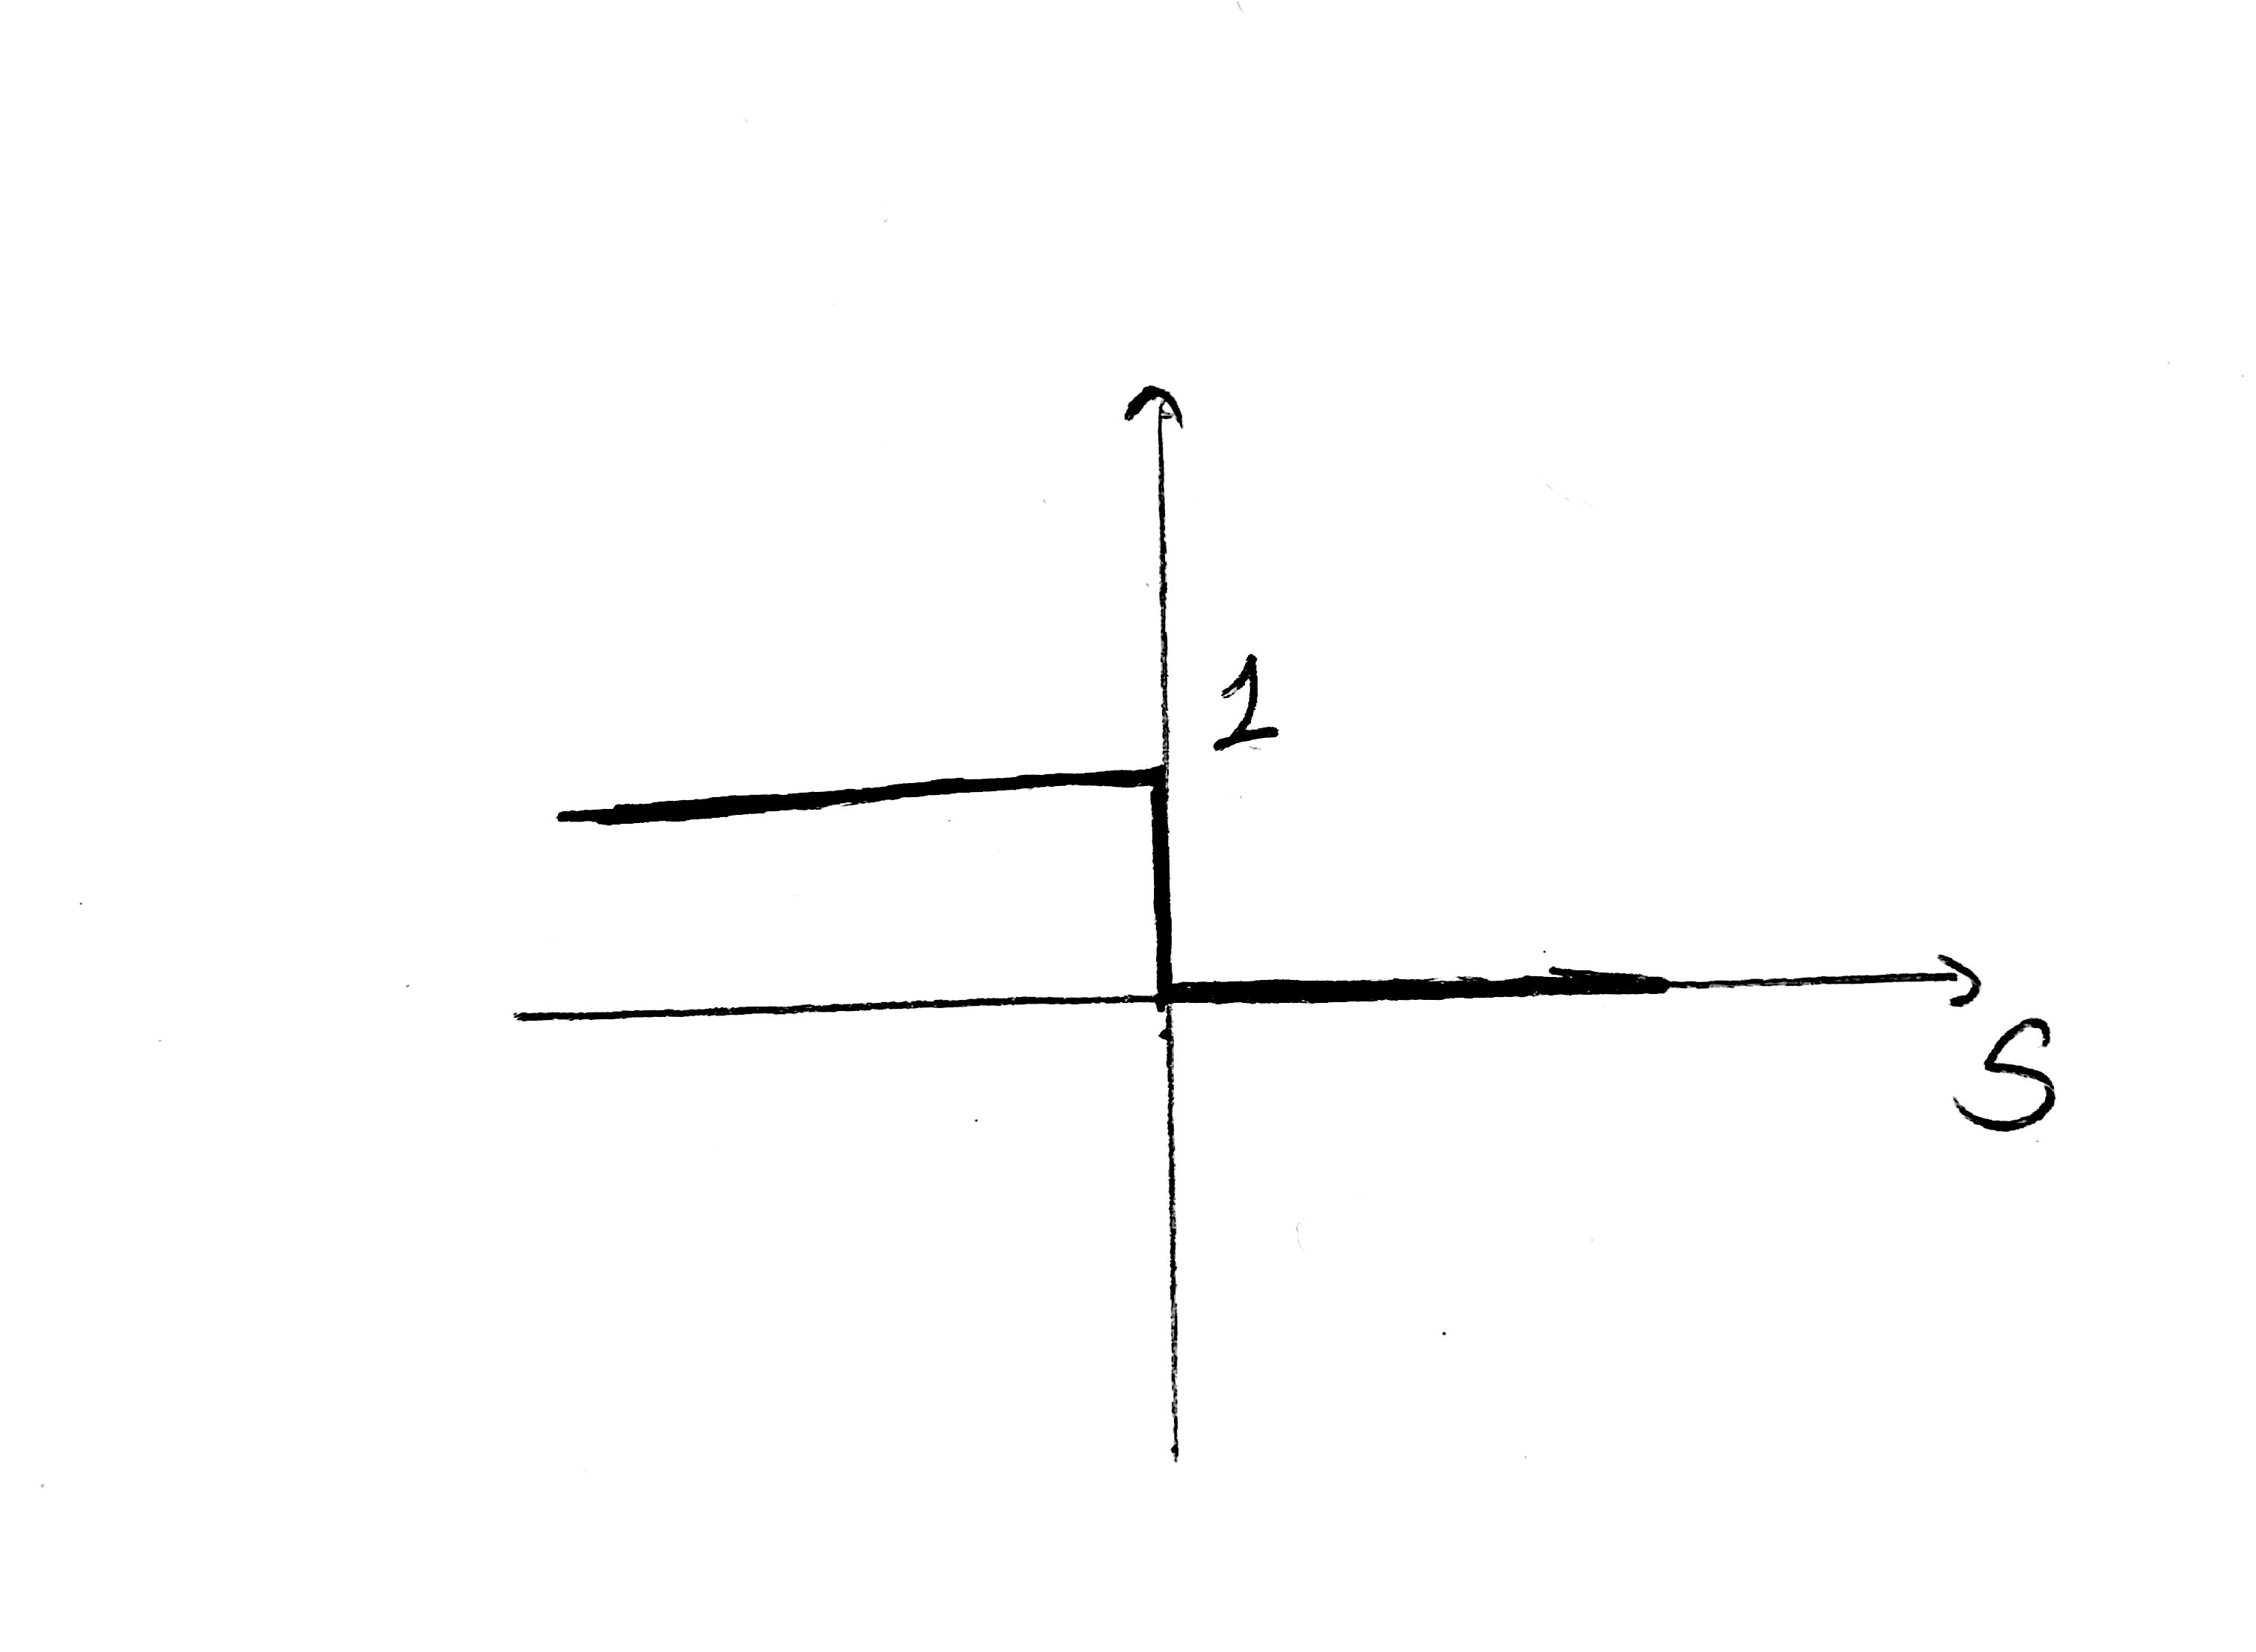
\includegraphics[width=120mm]{Non-covex.jpg}
\caption{ Non-covex form }
\end{figure}

In convex form, we need the graph to be:\\
\begin{figure}[H]
\centering
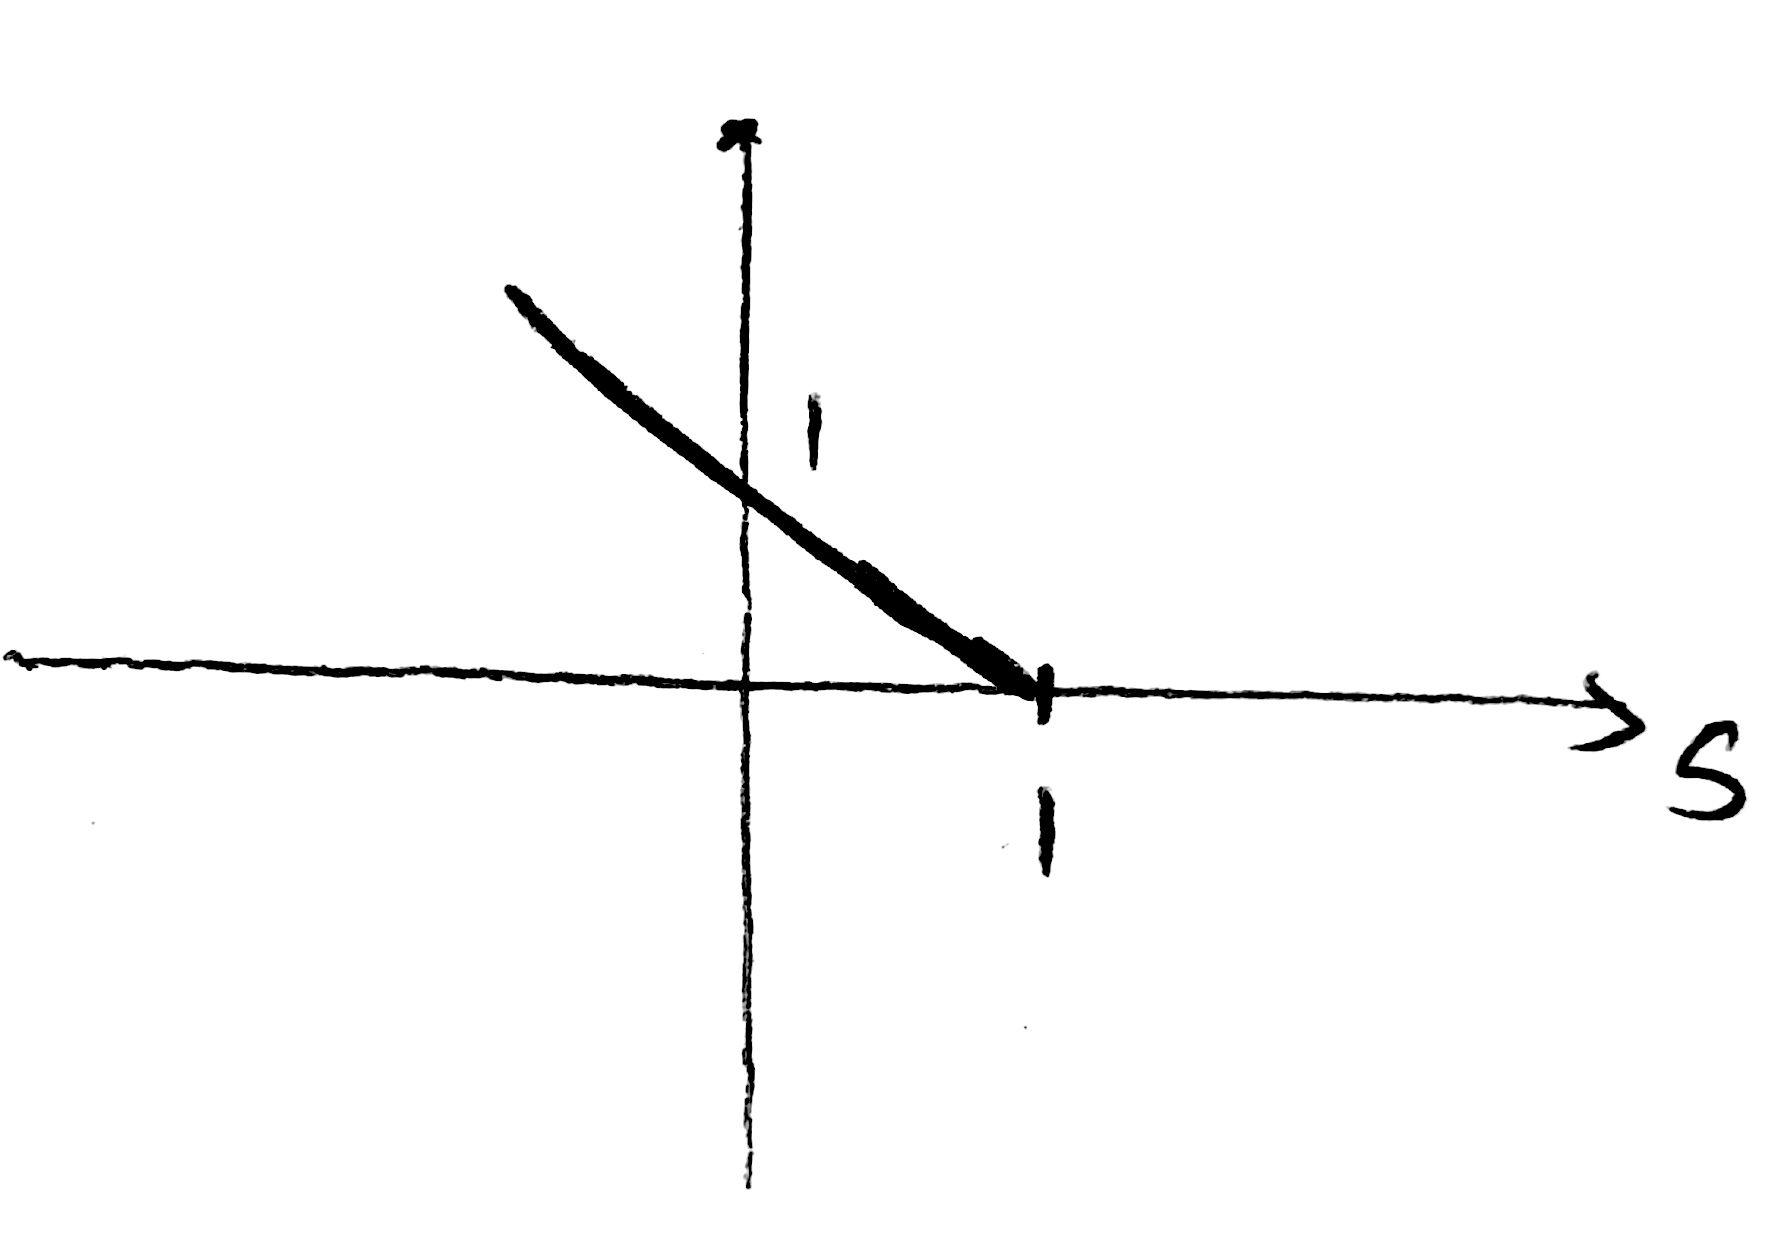
\includegraphics[width=120mm]{covex.jpg}
\caption{ Covex form}
\end{figure}


This is called convex upper bond, and such graph can be described as:
\[ \underset{w}{\operatorname{min}} \frac{C}{n} \sum_{i=1}^n \mathbbm{1} (w^T x_i y_i \leq 0) \;\;\;\;\; s.t. \; \|w\| \leq 1\]
Note: As $C$ goes to infinite, the soft-margin becomes hard-margin. Since $C$ stands for how much we tolerant the error. Since the $C-SVM$ is sometimes not that interpretable, we can use $\nu - SVM$ instead. Therefore we have:
\[\hat W \in \underset{W,\rho}{\operatorname{argmin}} \frac{1}{2} \|w\|^2 - \nu \rho + \frac{1}{n}\sum_{i=1}^n ( \rho - y_i w^T x_i )_+ \;\;\;\;\;\;\; \rho \geq 0\]
The $\nu\rho$ term says that we want a bigger $\rho$.
Referring to the diagram below, as $\rho$ increases, I am increasing the intersection $a$.
Theorm:
\[|{i|y_i \hat w^T x_i < \rho}| \leq | { i| \alpha_i = \frac{1}{n}}| \leq \nu n \leq |{i| \alpha_i > 0}| \leq | { i| y_i \hat w^T x_i \leq \rho}|\]
So $\nu n$ tells us how many erros I should have. A.k.a: the number of strict margin error is a subset of $\nu n$. Strict margin error are things within the margin boundary. ${i| y_i \hat w^T x_i \leq \rho}$ includes the points on the margin boundary. The proof of this theorm will be posted online.  
Theorm:\\
Take a soultion of $ \nu - SVM$, and let $\rho^*$ be the optimal $\rho$, that is larger than 0, then $C = \frac{1}{\rho^*}$ gives an equivalent problem. \\
The proof of this theorm is left as an exercise. 


\section{Statical Learning Theory}
We have been talking about something called Empirical Risk Minimization. \\
In decision theory (STAT 610/611), we often have some loss of our parameters, $l(w,y,x) \in \R$. e.g. $-\frac{1}{2}(w^Tx - y)^2$, and $-\mathbbm{1}(w^Txy \leq 0)$, so we ideally want to find:
\[w^* = \underset{w}{\operatorname{argmin}}\;\E[l(w,x,y)]\]
Note that $x$, $y$ are drawn from some distribution. \\
we can define the risk of $w$ to be:
\[R(w) = \E[l(w,x,y)]\]
But we don't have access to the distribution governing $(x,y)$; instead, we have $n$ i.i.d samples, and therefore we have:
\[\hat R (w) = \frac{1}{n} \sum_{i=1}^n l(w,x_i,y_i)\]
If we have a fixed $w$, what is the epxected value of $\hat R (w)$? \\
It is just $R(w)$ so we are just taking the average: $\;\E \;\hat R (w) = R(w)$.
The question is that when is optimizing $\hat R (w)$ good enough?\\
Let $R^* = \underset{w}{\operatorname{min}}\;\E\;[l(w,x,y)]$ be the optimal solution.\\
Let $\hat w = \underset{w}{\operatorname{argmin}} \hat R (w)$. \\
How do we relate $R(\hat w)$ to $R(w^*)$? a.k.a: Can we show that  $R(\hat w) - R(w^*)$ is small?\\
$R(\hat w)$ is called "generalization error".\\
Ex: binary classification \\
\[l(w,x,y) = \mathbbm{1} (w^T x y \leq 0) \Rightarrow R(\hat w)\]
This is the probability that $\hat w$ makes a mistake. \\
i.e. \[R(\hat w) = \;\E \;[\mathbbm{1}(\hat w^T xy \leq 0)] = P(\hat w^T xy \leq 0)= P(\hat w\; makes \; an \; error\]
$R(\hat w)$ is random, so we often want to consider $\E[R(w)]$ or we can also show that with high probability, $R(\hat w) \leq R(w^*) + \varepsilon$. a.k.a: $P(R(\hat w) > R(w^*)+ \varepsilon)$ is small.\\ 
\\
Theorm:\\
If $|\hat R (w) - R(w)| \leq \varepsilon \;\;\;\; \forall w$, then
\[ R(\hat w) \leq R(w^*) + 2 \varepsilon\]
if $\varepsilon = 0$, then $R(\hat w) = R(w^*)$. \\
Proof:\\
Note that $R(\hat w) - \hat r(\hat w) \leq \varepsilon$.\\
\[R(\hat w)-R(w^*) = R(\hat w) - \hat R (\hat w)+\hat R (\hat w) - R(w^*)\]
\[=R(\hat w) - \hat R(\hat w) + \hat R(\hat w) - R(w^*)+ \hat R(w^*)-\hat R(w^*)\]
\[=[R(\hat w) - \hat R(\hat w)]+[\hat R(\hat w) - \hat R (w^*)]+[\hat R(w^*) - R(w^*)]\]
\[\leq \varepsilon + 0 + \varepsilon\]
\[\leq 2 \varepsilon\]
For example, sample mean:\\
Let $x_i = 1$ with probability $p$, and $x_i = 0$ with probability $1-p$. 
\[\hat \mu = \underset{\mu}{\operatorname{argmin}} \frac{1}{n} \sum_{i=1}^n (\mu - x_i)^2 \]
\[\Rightarrow \hat \mu = \frac{1}{n} \sum_{i=1}^n x_i\]
\[R(\mu) = \;\E\; (\mu - x_i)^2 = var(x_i) + (\mu - p)^2\]
\[=p(1-p)+(\mu-p)^2\]
\[\hat R(\mu) = \frac{1}{n} \sum_{i=1}^n (\mu - x_i)^2 \]
Now we get:\\
\[\hat R(\mu) - R(\mu) = \frac{1}{n} \sum_{i=1}^n [(\mu - x_i)^2 - (p(1-p)+(\mu-p)^2)]\]
\[=\frac{1}{n} \sum_{i=1}^n[(\mu - p + p -x_i)^2 - R(\mu)]\]
\[=\frac{1}{n} \sum_{i=1}^n[(\mu-p)^2 + (p-x_i)^2 - R(\mu) + (\mu-p)(p-x_i)]\]
...... Finish next time.\\






\end{document}
